% Created by tikzDevice version 0.12.3 on 2020-05-11 12:44:46
% !TEX encoding = UTF-8 Unicode
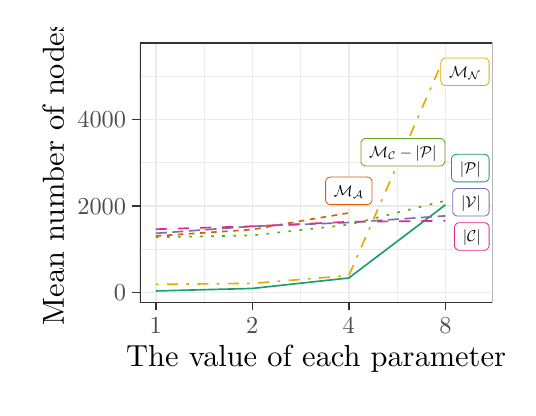
\begin{tikzpicture}[x=1pt,y=1pt]
\definecolor{fillColor}{RGB}{255,255,255}
\path[use as bounding box,fill=fillColor,fill opacity=0.00] (0,0) rectangle (173.45,130.09);
\begin{scope}
\path[clip] (  0.00,  0.00) rectangle (173.45,130.09);
\definecolor{drawColor}{RGB}{255,255,255}
\definecolor{fillColor}{RGB}{255,255,255}

\path[draw=drawColor,line width= 0.6pt,line join=round,line cap=round,fill=fillColor] (  0.00,  0.00) rectangle (173.45,130.09);
\end{scope}
\begin{scope}
\path[clip] ( 40.51, 30.69) rectangle (167.95,124.59);
\definecolor{fillColor}{RGB}{255,255,255}

\path[fill=fillColor] ( 40.51, 30.69) rectangle (167.95,124.59);
\definecolor{drawColor}{gray}{0.92}

\path[draw=drawColor,line width= 0.3pt,line join=round] ( 40.51, 50.03) --
	(167.95, 50.03);

\path[draw=drawColor,line width= 0.3pt,line join=round] ( 40.51, 81.30) --
	(167.95, 81.30);

\path[draw=drawColor,line width= 0.3pt,line join=round] ( 40.51,112.57) --
	(167.95,112.57);

\path[draw=drawColor,line width= 0.3pt,line join=round] ( 63.74, 30.69) --
	( 63.74,124.59);

\path[draw=drawColor,line width= 0.3pt,line join=round] ( 98.62, 30.69) --
	( 98.62,124.59);

\path[draw=drawColor,line width= 0.3pt,line join=round] (133.49, 30.69) --
	(133.49,124.59);

\path[draw=drawColor,line width= 0.6pt,line join=round] ( 40.51, 34.40) --
	(167.95, 34.40);

\path[draw=drawColor,line width= 0.6pt,line join=round] ( 40.51, 65.67) --
	(167.95, 65.67);

\path[draw=drawColor,line width= 0.6pt,line join=round] ( 40.51, 96.94) --
	(167.95, 96.94);

\path[draw=drawColor,line width= 0.6pt,line join=round] ( 46.30, 30.69) --
	( 46.30,124.59);

\path[draw=drawColor,line width= 0.6pt,line join=round] ( 81.18, 30.69) --
	( 81.18,124.59);

\path[draw=drawColor,line width= 0.6pt,line join=round] (116.05, 30.69) --
	(116.05,124.59);

\path[draw=drawColor,line width= 0.6pt,line join=round] (150.93, 30.69) --
	(150.93,124.59);
\definecolor{drawColor}{RGB}{27,158,119}

\path[draw=drawColor,line width= 0.6pt,line join=round] ( 46.30, 34.95) --
	( 81.18, 35.86) --
	(116.05, 39.64) --
	(150.93, 66.05);
\definecolor{drawColor}{RGB}{217,95,2}

\path[draw=drawColor,line width= 0.6pt,dash pattern=on 2pt off 2pt ,line join=round] ( 46.30, 54.81) --
	( 81.18, 57.14) --
	(101.58, 60.74) --
	(116.05, 63.15);
\definecolor{drawColor}{RGB}{117,112,179}

\path[draw=drawColor,line width= 0.6pt,dash pattern=on 4pt off 2pt ,line join=round] ( 46.30, 55.77) --
	( 81.18, 58.31) --
	(116.05, 59.68) --
	(150.93, 62.08);
\definecolor{drawColor}{RGB}{231,41,138}

\path[draw=drawColor,line width= 0.6pt,dash pattern=on 4pt off 4pt ,line join=round] ( 46.30, 57.27) --
	( 81.18, 58.33) --
	(116.05, 59.95) --
	(150.93, 60.30);
\definecolor{drawColor}{RGB}{102,166,30}

\path[draw=drawColor,line width= 0.6pt,dash pattern=on 1pt off 3pt ,line join=round] ( 46.30, 54.34) --
	( 81.18, 55.03) --
	(116.05, 58.92) --
	(150.93, 67.56);
\definecolor{drawColor}{RGB}{230,171,2}

\path[draw=drawColor,line width= 0.6pt,dash pattern=on 1pt off 3pt on 4pt off 3pt ,line join=round] ( 46.30, 37.33) --
	( 81.18, 37.69) --
	(116.05, 40.51) --
	(150.93,120.32);
\end{scope}
\begin{scope}
\path[clip] ( 40.51, 30.69) rectangle (167.95,124.59);

\path[] (158.55, 74.38) -- (150.93, 66.05);
\definecolor{drawColor}{RGB}{27,158,119}
\definecolor{fillColor}{RGB}{255,255,255}

\path[draw=drawColor,line width= 0.3pt,line join=round,line cap=round,fill=fillColor] (154.94, 74.38) --
	(164.94, 74.38) --
	(164.86, 74.38) --
	(165.15, 74.39) --
	(165.44, 74.45) --
	(165.71, 74.55) --
	(165.96, 74.70) --
	(166.19, 74.88) --
	(166.38, 75.10) --
	(166.54, 75.34) --
	(166.65, 75.61) --
	(166.72, 75.89) --
	(166.74, 76.18) --
	(166.74, 76.18) --
	(166.74, 82.51) --
	(166.74, 82.51) --
	(166.72, 82.80) --
	(166.65, 83.08) --
	(166.54, 83.35) --
	(166.38, 83.60) --
	(166.19, 83.81) --
	(165.96, 84.00) --
	(165.71, 84.14) --
	(165.44, 84.25) --
	(165.15, 84.30) --
	(164.94, 84.32) --
	(154.94, 84.32) --
	(155.16, 84.30) --
	(154.87, 84.32) --
	(154.58, 84.28) --
	(154.30, 84.20) --
	(154.04, 84.08) --
	(153.80, 83.91) --
	(153.59, 83.71) --
	(153.41, 83.48) --
	(153.28, 83.22) --
	(153.19, 82.94) --
	(153.14, 82.66) --
	(153.13, 82.51) --
	(153.13, 76.18) --
	(153.14, 76.33) --
	(153.14, 76.04) --
	(153.19, 75.75) --
	(153.28, 75.47) --
	(153.41, 75.22) --
	(153.59, 74.98) --
	(153.80, 74.78) --
	(154.04, 74.62) --
	(154.30, 74.49) --
	(154.58, 74.41) --
	(154.87, 74.38) --
	cycle;
\end{scope}
\begin{scope}
\path[clip] ( 40.51, 30.69) rectangle (167.95,124.59);
\definecolor{drawColor}{RGB}{27,158,119}

\node[text=black,anchor=base,inner sep=0pt, outer sep=0pt, scale=  0.57] at (159.94, 77.39) {$|\mathcal{P}|$};
\end{scope}
\begin{scope}
\path[clip] ( 40.51, 30.69) rectangle (167.95,124.59);
\definecolor{drawColor}{RGB}{117,112,179}
\definecolor{fillColor}{RGB}{255,255,255}

\path[draw=drawColor,line width= 0.3pt,line join=round,line cap=round,fill=fillColor] (155.41, 62.03) --
	(164.94, 62.03) --
	(164.86, 62.03) --
	(165.15, 62.04) --
	(165.44, 62.10) --
	(165.71, 62.20) --
	(165.96, 62.35) --
	(166.19, 62.53) --
	(166.38, 62.75) --
	(166.53, 63.00) --
	(166.65, 63.26) --
	(166.72, 63.55) --
	(166.74, 63.84) --
	(166.74, 63.84) --
	(166.74, 70.16) --
	(166.74, 70.16) --
	(166.72, 70.45) --
	(166.65, 70.74) --
	(166.53, 71.00) --
	(166.38, 71.25) --
	(166.19, 71.47) --
	(165.96, 71.65) --
	(165.71, 71.80) --
	(165.44, 71.90) --
	(165.15, 71.96) --
	(164.94, 71.97) --
	(155.41, 71.97) --
	(155.63, 71.96) --
	(155.34, 71.97) --
	(155.05, 71.93) --
	(154.77, 71.85) --
	(154.51, 71.73) --
	(154.27, 71.56) --
	(154.06, 71.36) --
	(153.88, 71.13) --
	(153.75, 70.87) --
	(153.65, 70.60) --
	(153.61, 70.31) --
	(153.60, 70.16) --
	(153.60, 63.84) --
	(153.61, 63.98) --
	(153.61, 63.69) --
	(153.65, 63.40) --
	(153.75, 63.13) --
	(153.88, 62.87) --
	(154.06, 62.64) --
	(154.27, 62.44) --
	(154.51, 62.27) --
	(154.77, 62.15) --
	(155.05, 62.07) --
	(155.34, 62.03) --
	cycle;
\end{scope}
\begin{scope}
\path[clip] ( 40.51, 30.69) rectangle (167.95,124.59);
\definecolor{drawColor}{RGB}{117,112,179}

\node[text=black,anchor=base,inner sep=0pt, outer sep=0pt, scale=  0.57] at (160.17, 65.04) {$|\mathcal{V}|$};
\end{scope}
\begin{scope}
\path[clip] ( 40.51, 30.69) rectangle (167.95,124.59);
\definecolor{drawColor}{RGB}{231,41,138}
\definecolor{fillColor}{RGB}{255,255,255}

\path[draw=drawColor,line width= 0.3pt,line join=round,line cap=round,fill=fillColor] (156.04, 49.68) --
	(164.94, 49.68) --
	(164.86, 49.68) --
	(165.15, 49.69) --
	(165.44, 49.75) --
	(165.71, 49.85) --
	(165.96, 50.00) --
	(166.19, 50.18) --
	(166.38, 50.40) --
	(166.54, 50.65) --
	(166.65, 50.91) --
	(166.72, 51.20) --
	(166.74, 51.49) --
	(166.74, 51.49) --
	(166.74, 57.81) --
	(166.74, 57.81) --
	(166.72, 58.10) --
	(166.65, 58.39) --
	(166.54, 58.65) --
	(166.38, 58.90) --
	(166.19, 59.12) --
	(165.96, 59.30) --
	(165.71, 59.45) --
	(165.44, 59.55) --
	(165.15, 59.61) --
	(164.94, 59.62) --
	(156.04, 59.62) --
	(156.26, 59.61) --
	(155.96, 59.62) --
	(155.68, 59.58) --
	(155.40, 59.50) --
	(155.13, 59.38) --
	(154.89, 59.21) --
	(154.69, 59.01) --
	(154.51, 58.78) --
	(154.38, 58.52) --
	(154.28, 58.25) --
	(154.24, 57.96) --
	(154.23, 57.81) --
	(154.23, 51.49) --
	(154.24, 51.63) --
	(154.24, 51.34) --
	(154.28, 51.05) --
	(154.38, 50.78) --
	(154.51, 50.52) --
	(154.69, 50.29) --
	(154.89, 50.09) --
	(155.13, 49.92) --
	(155.40, 49.80) --
	(155.68, 49.72) --
	(155.96, 49.68) --
	cycle;
\end{scope}
\begin{scope}
\path[clip] ( 40.51, 30.69) rectangle (167.95,124.59);
\definecolor{drawColor}{RGB}{231,41,138}

\node[text=black,anchor=base,inner sep=0pt, outer sep=0pt, scale=  0.57] at (160.49, 52.69) {$|\mathcal{C}|$};
\end{scope}
\begin{scope}
\path[clip] ( 40.51, 30.69) rectangle (167.95,124.59);

\path[] (139.49, 80.12) -- (150.93, 67.56);
\definecolor{drawColor}{RGB}{102,166,30}
\definecolor{fillColor}{RGB}{255,255,255}

\path[draw=drawColor,line width= 0.3pt,line join=round,line cap=round,fill=fillColor] (122.22, 80.12) --
	(148.97, 80.12) --
	(148.89, 80.12) --
	(149.18, 80.13) --
	(149.47, 80.19) --
	(149.74, 80.29) --
	(149.99, 80.44) --
	(150.22, 80.62) --
	(150.41, 80.84) --
	(150.57, 81.08) --
	(150.68, 81.35) --
	(150.75, 81.63) --
	(150.77, 81.92) --
	(150.77, 81.92) --
	(150.77, 88.25) --
	(150.77, 88.25) --
	(150.75, 88.54) --
	(150.68, 88.82) --
	(150.57, 89.09) --
	(150.41, 89.34) --
	(150.22, 89.55) --
	(149.99, 89.74) --
	(149.74, 89.88) --
	(149.47, 89.99) --
	(149.18, 90.05) --
	(148.97, 90.06) --
	(122.22, 90.06) --
	(122.44, 90.05) --
	(122.15, 90.06) --
	(121.86, 90.02) --
	(121.58, 89.94) --
	(121.32, 89.82) --
	(121.08, 89.65) --
	(120.87, 89.45) --
	(120.70, 89.22) --
	(120.56, 88.96) --
	(120.47, 88.68) --
	(120.42, 88.40) --
	(120.42, 88.25) --
	(120.42, 81.92) --
	(120.42, 82.07) --
	(120.42, 81.78) --
	(120.47, 81.49) --
	(120.56, 81.21) --
	(120.70, 80.96) --
	(120.87, 80.72) --
	(121.08, 80.52) --
	(121.32, 80.36) --
	(121.58, 80.23) --
	(121.86, 80.15) --
	(122.15, 80.12) --
	cycle;
\end{scope}
\begin{scope}
\path[clip] ( 40.51, 30.69) rectangle (167.95,124.59);
\definecolor{drawColor}{RGB}{102,166,30}

\node[text=black,anchor=base,inner sep=0pt, outer sep=0pt, scale=  0.57] at (135.59, 83.13) {$\mathcal{M}_{\mathcal{C}}-|\mathcal{P}|$};
\end{scope}
\begin{scope}
\path[clip] ( 40.51, 30.69) rectangle (167.95,124.59);
\definecolor{drawColor}{RGB}{230,171,2}
\definecolor{fillColor}{RGB}{255,255,255}

\path[draw=drawColor,line width= 0.3pt,line join=round,line cap=round,fill=fillColor] (151.08,109.18) --
	(164.94,109.18) --
	(164.86,109.18) --
	(165.15,109.19) --
	(165.44,109.25) --
	(165.71,109.36) --
	(165.96,109.50) --
	(166.19,109.68) --
	(166.38,109.90) --
	(166.54,110.15) --
	(166.65,110.42) --
	(166.72,110.70) --
	(166.74,110.99) --
	(166.74,110.99) --
	(166.74,117.32) --
	(166.74,117.32) --
	(166.72,117.61) --
	(166.65,117.89) --
	(166.54,118.16) --
	(166.38,118.40) --
	(166.19,118.62) --
	(165.96,118.80) --
	(165.71,118.95) --
	(165.44,119.05) --
	(165.15,119.11) --
	(164.94,119.12) --
	(151.08,119.12) --
	(151.30,119.11) --
	(151.01,119.12) --
	(150.72,119.09) --
	(150.44,119.01) --
	(150.18,118.88) --
	(149.94,118.72) --
	(149.73,118.51) --
	(149.56,118.28) --
	(149.42,118.02) --
	(149.33,117.75) --
	(149.28,117.46) --
	(149.28,117.32) --
	(149.28,110.99) --
	(149.28,111.13) --
	(149.28,110.84) --
	(149.33,110.56) --
	(149.42,110.28) --
	(149.56,110.02) --
	(149.73,109.79) --
	(149.94,109.59) --
	(150.18,109.42) --
	(150.44,109.30) --
	(150.72,109.22) --
	(151.01,109.18) --
	cycle;
\end{scope}
\begin{scope}
\path[clip] ( 40.51, 30.69) rectangle (167.95,124.59);
\definecolor{drawColor}{RGB}{230,171,2}

\node[text=black,anchor=base,inner sep=0pt, outer sep=0pt, scale=  0.57] at (158.01,112.19) {$\mathcal{M}_{\mathcal{N}}$};
\end{scope}
\begin{scope}
\path[clip] ( 40.51, 30.69) rectangle (167.95,124.59);
\definecolor{drawColor}{RGB}{217,95,2}
\definecolor{fillColor}{RGB}{255,255,255}

\path[draw=drawColor,line width= 0.3pt,line join=round,line cap=round,fill=fillColor] (109.46, 66.16) --
	(122.64, 66.16) --
	(122.57, 66.16) --
	(122.86, 66.17) --
	(123.15, 66.23) --
	(123.42, 66.33) --
	(123.67, 66.48) --
	(123.90, 66.66) --
	(124.09, 66.88) --
	(124.24, 67.12) --
	(124.36, 67.39) --
	(124.43, 67.67) --
	(124.45, 67.96) --
	(124.45, 67.96) --
	(124.45, 74.29) --
	(124.45, 74.29) --
	(124.43, 74.58) --
	(124.36, 74.86) --
	(124.24, 75.13) --
	(124.09, 75.38) --
	(123.90, 75.60) --
	(123.67, 75.78) --
	(123.42, 75.92) --
	(123.15, 76.03) --
	(122.86, 76.09) --
	(122.64, 76.10) --
	(109.46, 76.10) --
	(109.68, 76.09) --
	(109.39, 76.10) --
	(109.10, 76.06) --
	(108.82, 75.98) --
	(108.56, 75.86) --
	(108.32, 75.69) --
	(108.11, 75.49) --
	(107.93, 75.26) --
	(107.80, 75.00) --
	(107.71, 74.72) --
	(107.66, 74.44) --
	(107.65, 74.29) --
	(107.65, 67.96) --
	(107.66, 68.11) --
	(107.66, 67.82) --
	(107.71, 67.53) --
	(107.80, 67.26) --
	(107.93, 67.00) --
	(108.11, 66.77) --
	(108.32, 66.56) --
	(108.56, 66.40) --
	(108.82, 66.27) --
	(109.10, 66.19) --
	(109.39, 66.16) --
	cycle;
\end{scope}
\begin{scope}
\path[clip] ( 40.51, 30.69) rectangle (167.95,124.59);
\definecolor{drawColor}{RGB}{217,95,2}

\node[text=black,anchor=base,inner sep=0pt, outer sep=0pt, scale=  0.57] at (116.05, 69.17) {$\mathcal{M}_{\mathcal{A}}$};
\definecolor{drawColor}{gray}{0.20}

\path[draw=drawColor,line width= 0.6pt,line join=round,line cap=round] ( 40.51, 30.69) rectangle (167.95,124.59);
\end{scope}
\begin{scope}
\path[clip] (  0.00,  0.00) rectangle (173.45,130.09);
\definecolor{drawColor}{gray}{0.30}

\node[text=drawColor,anchor=base east,inner sep=0pt, outer sep=0pt, scale=  0.88] at ( 35.56, 31.37) {0};

\node[text=drawColor,anchor=base east,inner sep=0pt, outer sep=0pt, scale=  0.88] at ( 35.56, 62.64) {2000};

\node[text=drawColor,anchor=base east,inner sep=0pt, outer sep=0pt, scale=  0.88] at ( 35.56, 93.91) {4000};
\end{scope}
\begin{scope}
\path[clip] (  0.00,  0.00) rectangle (173.45,130.09);
\definecolor{drawColor}{gray}{0.20}

\path[draw=drawColor,line width= 0.6pt,line join=round] ( 37.76, 34.40) --
	( 40.51, 34.40);

\path[draw=drawColor,line width= 0.6pt,line join=round] ( 37.76, 65.67) --
	( 40.51, 65.67);

\path[draw=drawColor,line width= 0.6pt,line join=round] ( 37.76, 96.94) --
	( 40.51, 96.94);
\end{scope}
\begin{scope}
\path[clip] (  0.00,  0.00) rectangle (173.45,130.09);
\definecolor{drawColor}{gray}{0.20}

\path[draw=drawColor,line width= 0.6pt,line join=round] ( 46.30, 27.94) --
	( 46.30, 30.69);

\path[draw=drawColor,line width= 0.6pt,line join=round] ( 81.18, 27.94) --
	( 81.18, 30.69);

\path[draw=drawColor,line width= 0.6pt,line join=round] (116.05, 27.94) --
	(116.05, 30.69);

\path[draw=drawColor,line width= 0.6pt,line join=round] (150.93, 27.94) --
	(150.93, 30.69);
\end{scope}
\begin{scope}
\path[clip] (  0.00,  0.00) rectangle (173.45,130.09);
\definecolor{drawColor}{gray}{0.30}

\node[text=drawColor,anchor=base,inner sep=0pt, outer sep=0pt, scale=  0.88] at ( 46.30, 19.68) {1};

\node[text=drawColor,anchor=base,inner sep=0pt, outer sep=0pt, scale=  0.88] at ( 81.18, 19.68) {2};

\node[text=drawColor,anchor=base,inner sep=0pt, outer sep=0pt, scale=  0.88] at (116.05, 19.68) {4};

\node[text=drawColor,anchor=base,inner sep=0pt, outer sep=0pt, scale=  0.88] at (150.93, 19.68) {8};
\end{scope}
\begin{scope}
\path[clip] (  0.00,  0.00) rectangle (173.45,130.09);
\definecolor{drawColor}{RGB}{0,0,0}

\node[text=drawColor,anchor=base,inner sep=0pt, outer sep=0pt, scale=  1.10] at (104.23,  7.64) {The value of each parameter};
\end{scope}
\begin{scope}
\path[clip] (  0.00,  0.00) rectangle (173.45,130.09);
\definecolor{drawColor}{RGB}{0,0,0}

\node[text=drawColor,rotate= 90.00,anchor=base,inner sep=0pt, outer sep=0pt, scale=  1.10] at ( 13.08, 77.64) {Mean number of nodes};
\end{scope}
\end{tikzpicture}
